
%%%%%%%%%%%%%%%%%%%%%%%%%%%%%%%%%%%%%%%%%%%%%%%%
\begin{figure}[h!]
  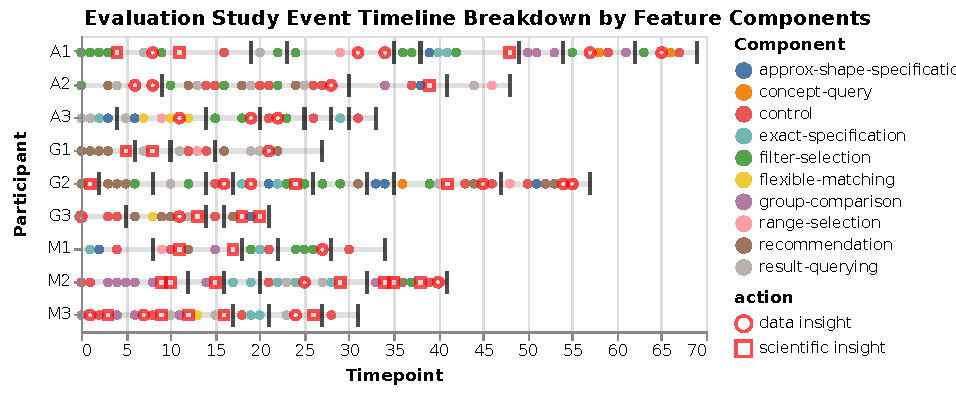
\includegraphics[width=\linewidth]{figures/evalstudytimeline.pdf}
  \caption{Timeline of event code and component usage, with every timepoint as an event on the x axis. For clarity, we hide most of the event coding labels other than the insight labels. Black vertical tick indicates a session break, signaling the beginning of a new line of inquiry.}\label{fig:evalstudytimeline}
\end{figure}
In Figure~\ref{fig:evalstudytimeline}, we map the features to components based on the taxonomy described in Figure~\ref{fig:taxonomy} to plot the timeline of event codes and component usage for each participant.
%%%%%%%%%%%%%%%%%%%%%%%%%%%%%%%%%%%%%%%%%%%%%%%%

%%%%%%%%%%%%%%%%%%%%%%%%%%%%%%%%%%%%%%%%%%%%%%%%
